\documentclass[a4paper]{article}
\usepackage{fullpage}
\usepackage{hyperref}
\usepackage{graphicx}
\title{Scenario Editor}
%\author{Group 3 of the A Search And Rescue Context Project}
\date{}
\begin{document}
\maketitle
\newpage

\tableofcontents
\newpage

\section{Introduction}
This document describes how to make use of the Scenario Editor (Figure 1). When you open the editor, you see two main parts:
\begin{enumerate}
\item The Configuration panel, which is used to create, open and save configuration files.
\item The Entity panel, where a list of bots and a list of e-partners are being displayed. Here you can create, modify, rename and delete bots and e-partners.
\end{enumerate}

\begin{figure}[h]
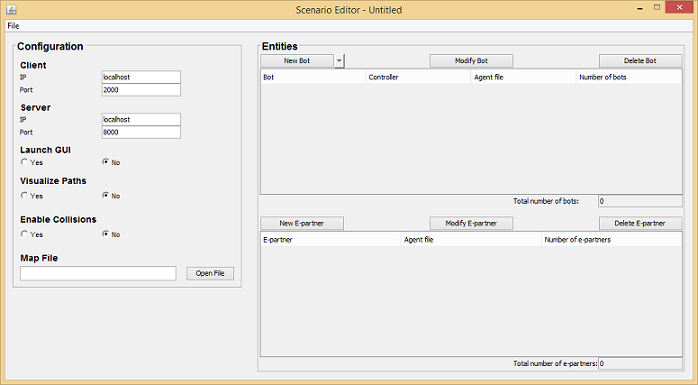
\includegraphics{editor.png}
\caption{Scenario Editor}
\end{figure}

\section{General use}
At the top of the editor you can see a $File$ menu. If you click on that, you get the options to create a new configuration, save your configuration, open a configuration and to exit the editor.

On the left side of the editor you can configure a scenario as you like. The Client IP, the Client Port, the Server IP and the Server Port should already contain the default values. You can change them if you need to. You can also indicate whether you want to open a GUI. If you have a Map file you want to use, you can import it by selecting the $Open$ $file$ button at the right section.

On the right side of the editor you can create, modify, rename and delete bots and e-partners. There also are a list of bots and a list of e-partners that are created, and below each list there is an indication of how many bots or e-partners are created in total.
\pagebreak
\section{Configuration Panel}
A picture of the configuration panel can be found in figure 2.
\begin{figure}[h]
\begin{center}
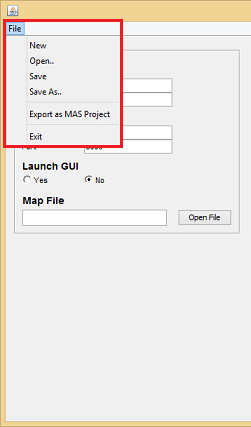
\includegraphics{config.png}
\end{center}
\caption{Configuration Panel}
\end{figure}
\subsection{New configuration file}
To create a new configuration file, select $File$ $\to$ $New$ in the menu bar. You will now get a new configuration with the default values. Creating a new configuration will reset all previous changes you have made, so make sure you save your current configuration first if you want to keep it.

\subsection{Save configuration file}
To save your configuration file, select $File$ $\to$ $Save$ in the menu bar. If your file hasn't been saved before, a screen will pop up where you can select the folder you want to save your file to and enter the file name you want to use. Once you have selected the right folder and entered the file name, click the $Save$ button.

\subsection{Save configuration file as}
To save your configuration in a new file, select $File$ $\to$ $Save$ $As$ in the menu bar. A screen will pop up where you can select the folder you want to save your file to and enter the file name you want to use. Once you have selected the right folder and entered the file name, click the $Save$ button.

\subsection{Open configuration file}
To open an existing configuration file, select $File$ $\to$ $Open$ in the menu bar. A screen will pop up where you can select the folder where the configuration file is saved to. Once you have selected the right folder, select the file and click the $Open$ button.

\section{Entity Panel}
The entity panel exists of 2 parts; the top part shows the bot options and the bottom part shows the e-partner options. A picture of the entity panel can be found in figure 3.
\begin{figure}[h]
\begin{center}
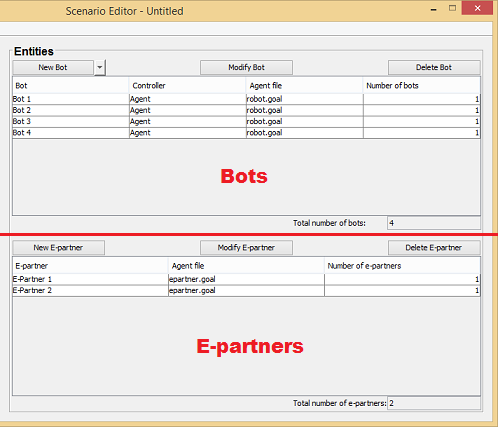
\includegraphics{bot.png}
\end{center}
\caption{Entity Panel}
\end{figure}
\subsection{Create new bot}
To create a new bot, click the $New$ $Bot$ button. A new bot will appear in the bot list.\\
If you want to create a standard bot (which already has default values), click on the arrow next to the $New$ $Bot$ button. A menu will drop down where you can select one of the standard bots. If you click on a bot, the bot will appear in the bot list.
%The Bot Store will open in a new window where you can create your bot.

\subsection{Modify bot}
To modify a bot, select the bot you want to modify in the bot list and click the $Modify$ $Bot$ button. The Bot Store will open in a new window where you can modify your bot.

\subsection{Change controller type}
To change how a bot is controlled, you can either use the $Modify$ $Bot$ button to change it in the Bot Store, or you can change it in the scenario editor. To change the controller type in the scenario editor, select the bot you want to change and click on its $Controller$ column. You should now be able to choose the controller type.

\subsection{Rename bot}
To rename a bot, you can either use the $Modify$ $Bot$ button to change it in the Bot Store, or you can change it in the scenario editor. To rename in the scenario editor, select the bot you want to rename in the list with bots. Double click the bots name and enter a new name. %Enter the new name in the textfield above the $Rename$ $bot$ button and click the $Rename$ $bot$ button.

\subsection{Delete bot}
To delete a bot, select the bot you want to delete in the list with bots and click the $Delete$ $Bot$ button.

\subsection{Create new e-partner}
To create a new e-partner, click the $New$ $E-partner$ button. A new e-partner will appear in the e-partner list.%The Bot Store will open in a new window where you can create your bot.

\subsection{Modify e-partner}
To modify an e-partner, select the e-partner you want to modify in the e-partner list and click the $Modify$ $E-partner$ button. A new window will open where you can modify the properties of the e-partner.

\subsection{Rename e-partner}
To rename an e-partner, select the e-partner you want to rename in the list with e-partners. Double click the e-partners name and enter a new name. %Enter the new name in the textfield above the $Rename$ $bot$ button and click the $Rename$ $bot$ button.

\subsection{Delete e-partner}
To delete an e-partner, select the e-partner you want to delete in the e-partner list and click the $Delete$ $E-partner$ button.

\end{document}